% DSB overall technical solution: offline training/export + online ROS2 TensorRT inference.
% Compile from DSB/docs: pdflatex dsb_tech_solution.tex  (or tectonic -X compile)
\documentclass[tikz,border=8pt]{standalone}

\usepackage{fontspec}
\setmainfont{Noto Sans CJK SC}
\usepackage{graphicx}
\usetikzlibrary{arrows.meta, backgrounds, calc, fit, positioning, shapes.geometric}

\definecolor{camA}{HTML}{2A78D6}
\definecolor{lidA}{HTML}{1BAF7A}
\definecolor{fusA}{HTML}{EB6834}
\definecolor{trtA}{HTML}{6250D6}
\definecolor{scnA}{HTML}{0E8FA8}
\definecolor{inkA}{HTML}{262626}
\definecolor{mutA}{HTML}{6B6B6B}

\tikzset{
  blk/.style={draw=inkA!70, line width=0.45pt, rounded corners=2.5pt,
    align=center, font=\small, inner sep=3pt, minimum height=0.95cm,
    text=inkA, fill=white},
  data/.style={blk, fill=black!5, draw=inkA!55},
  train/.style={blk, fill=camA!10, draw=camA!70},
  export/.style={blk, fill=fusA!12, draw=fusA!80},
  online/.style={blk, fill=lidA!10, draw=lidA!70},
  engine/.style={blk, fill=trtA!10, draw=trtA!75},
  scnnode/.style={blk, fill=scnA!10, draw=scnA!75},
  io/.style={blk, fill=black!4, draw=inkA!55},
  arr/.style={-{Stealth[length=2.1mm,width=1.5mm]}, line width=0.65pt, draw=inkA!75},
  darr/.style={arr, dashed},
  tag/.style={font=\scriptsize, text=mutA},
  grp/.style={draw=mutA!70, dashed, line width=0.6pt, rounded corners=6pt, inner sep=8pt},
  hdr/.style={font=\normalsize\bfseries, text=inkA, anchor=west},
  note/.style={font=\scriptsize, text=mutA, align=left},
}

\begin{document}
\begin{tikzpicture}

% ================================================================ OFFLINE
\node[data, text width=3.2cm] (data) at (0,15)
  {\textbf{nuScenes 数据}\\6 相机 + LiDAR + GT\\标定/外参};
\node[train, text width=3.6cm] (train) at (4.6,15)
  {\textbf{训练}\\Swin-T + SparseEncoder\\+ ConvFuser + heads\\det / seg / occ 配置};
\node[data] (ckpt) at (9.2,15) {\textbf{checkpoint}\\*.pth};
\node[export, text width=3.6cm] (onnx) at (13.6,15)
  {\textbf{ONNX 导出}\\export.py\\5 张图（含 SCN）};
\node[export, text width=3.6cm] (trtbuild) at (18.4,15)
  {\textbf{TRT 构建}\\export\_trt.sh\\4 个 fp16 plan};
\node[data, text width=4.2cm] (artifact) at (23.2,15)
  {\textbf{部署产物}\\model/<name>/build/\\*.plan\\lidar.backbone.xyz.onnx};

\node[data, text width=3.2cm] (calib) at (0,10.2)
  {\textbf{外参标定}\\fast\_calib\\camera2lidar / K / aug};

\draw[arr] (data) -- (train);
\draw[arr] (train) -- (ckpt);
\draw[arr] (ckpt) -- (onnx);
\draw[arr] (onnx) -- (trtbuild);
\draw[arr] (trtbuild) -- (artifact);
\draw[darr] (calib.north) -- (data.south);
\node[tag, anchor=west] at (0.25,11.8) {标定参与训练与在线推理};

% ================================================================ ONLINE INPUTS
\node[inner sep=1pt, draw=inkA!40, line width=0.5pt, rounded corners=2pt, fill=white] (campic) at (0,5.6)
  {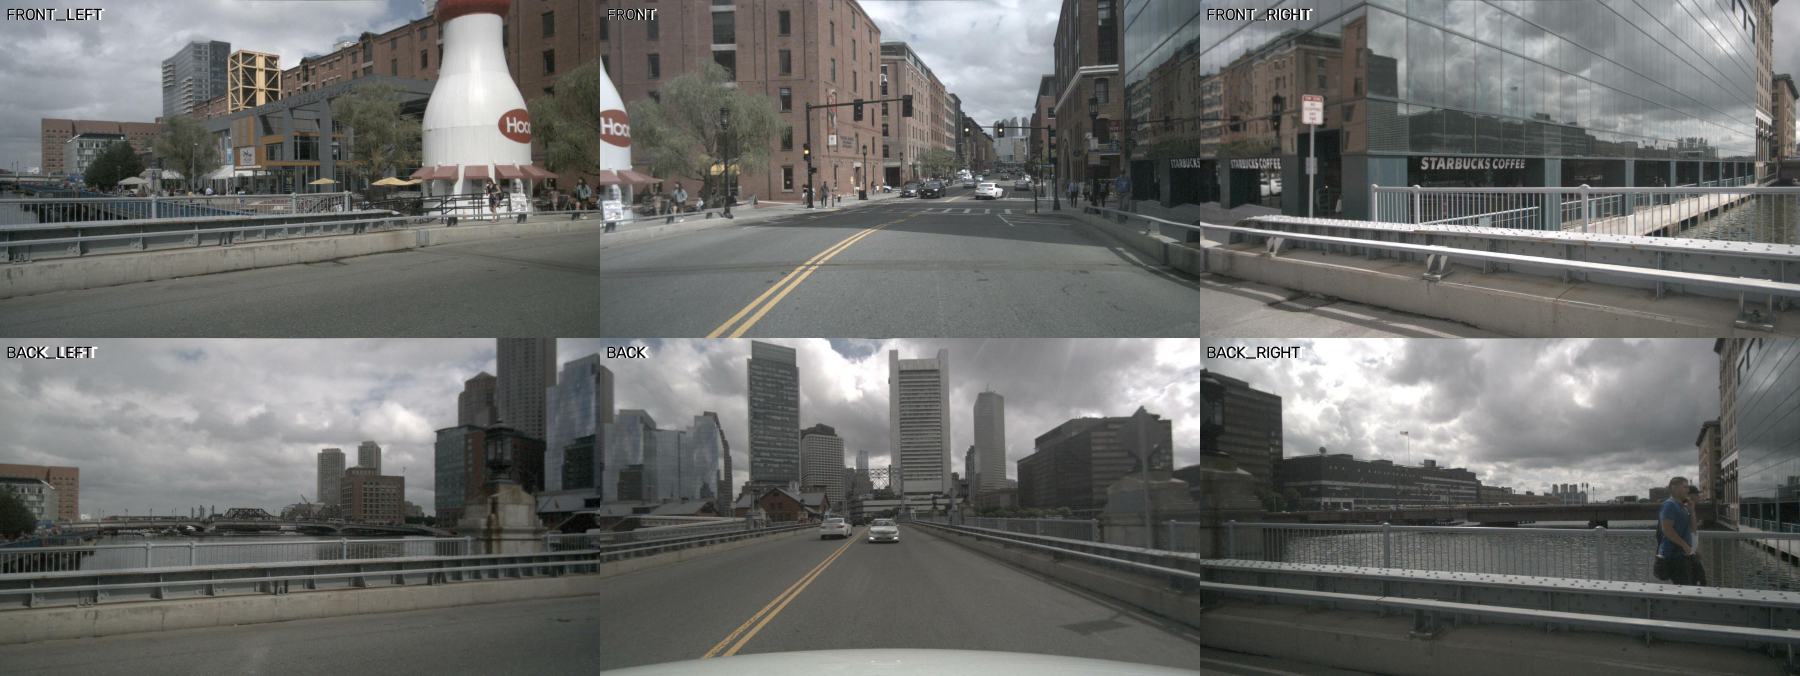
\includegraphics[width=3.2cm]{../3rdparty/deeplearning/docs/figs/cameras.png}};
\node[tag, anchor=north] at (0,4.85) {6$\times$ 相机 30 Hz / 1600$\times$900};

\node[inner sep=1pt, draw=inkA!40, line width=0.5pt, rounded corners=2pt, fill=black] (lidarpic) at (0,2.8)
  {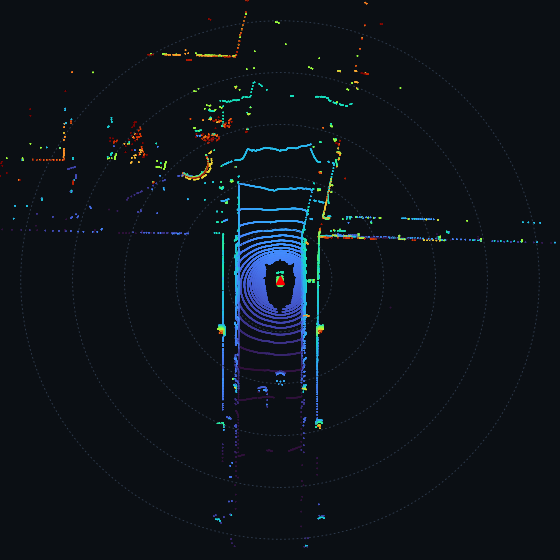
\includegraphics[width=1.6cm]{../3rdparty/deeplearning/docs/figs/lidar_bev.png}};
\node[tag, anchor=north] at (0,1.85) {LiDAR 10 Hz / $N\times5$};

\node[data, text width=2.4cm] (extr) at (2.7,4.0)
  {\textbf{外参}\\6$\times$4$\times$4\\camera2lidar / K\\lidar2image / aug};

% ================================================================ ONLINE NODE
\node[online, text width=2.9cm] (sync) at (6.0,4.0)
  {\textbf{时间戳同步}\\LiDAR 触发\\最近邻 $\le$ 50 ms\\缓存 3 帧};
\node[online, text width=3.0cm] (pre) at (9.8,4.0)
  {\textbf{预处理}\\RGB $\to$ 704$\times$256\\点云 $\to$ half $N\times5$};

\node[engine, text width=3.2cm] (cb) at (14.0,5.9)
  {\textbf{camera.backbone}\\Swin-T + FPN + DepthNet\\{[TRT]}};
\node[engine, text width=3.2cm] (vt) at (17.8,5.9)
  {\textbf{camera.vtransform}\\bev\_pool + downsample\\{[TRT + CUDA]}};
\node[scnnode, text width=3.0cm] (scn) at (14.0,2.2)
  {\textbf{SCN}\\voxelize + sparse conv\\{[libspconv]}};
\node[engine, text width=3.4cm] (fuser) at (21.4,4.0)
  {\textbf{fuser}\\ConvFuser + SECOND/FPN\\{[TRT]}};
\node[engine, text width=3.0cm] (head) at (25.2,4.0)
  {\textbf{head.bbox}\\TransFusion\\{[TRT]}};

\node[online, text width=3.2cm] (post) at (28.9,4.0)
  {\textbf{解码 + 发布}\\BoundingBoxArray\\MarkerArray (RViz)};

% ================================================================ ONLINE FLOW
\draw[arr] (campic.east) -- (sync.west);
\draw[arr] (lidarpic.east) -- (sync.south west);
\draw[arr] (extr.east) -- (sync.west);
\draw[arr] (sync) -- (pre);
\draw[arr] (pre.east) -| (cb.south);
\draw[arr] (pre.east) -| (scn.west);
\draw[arr] (cb) -- (vt);
\draw[arr] (vt.east) -| (fuser.north);
\draw[arr] (scn.east) -| (fuser.south);
\draw[arr] (fuser) -- (head);
\draw[arr] (head) -- (post);
\draw[arr] (artifact.south) -- (25.2,8.2) -- (head.north);
\node[tag, rotate=90] at (24.9,11.6) {plans / SCN onnx};

% ================================================================ OUTPUT
\node[inner sep=1.5pt, draw=inkA!40, line width=0.5pt, rounded corners=3pt, fill=white] (out) at (33.0,4.0)
  {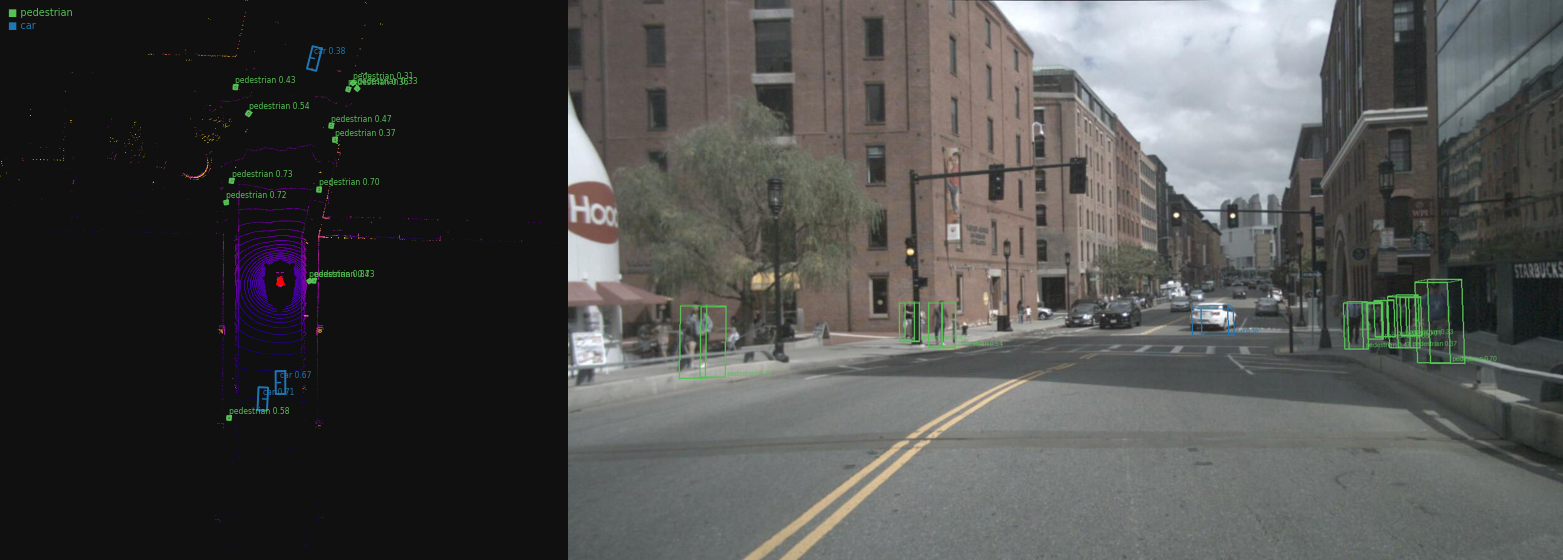
\includegraphics[width=4.6cm]{../3rdparty/deeplearning/docs/figs/det_result.png}};
\draw[arr] (post.east) -- (out.west);
\node[tag, anchor=north] at (33.0,2.9) {检测结果（示例帧）};

% ================================================================ notes / groups
\begin{scope}[on background layer]
  \node[grp, fit=(data)(train)(ckpt)(onnx)(trtbuild)(artifact),
        label={[tag]above:离线：训练与导出}] {};
  \node[grp, fit=(campic)(lidarpic)(extr)(sync)(pre)(cb)(vt)(scn)(fuser)(head)(post),
        label={[tag]above:在线：ROS2 + TensorRT（LiDAR 触发，单槽队列 + 工作线程）}] {};
\end{scope}

\node[note, anchor=north west, text width=15cm] at (-1.4,0.9)
  {\textbf{同步/吞吐：}相机 30 Hz、LiDAR 10 Hz；每帧 LiDAR 为 6 路相机选最近时间戳，
  偏差超过 50 ms 丢帧；同步帧进入单槽队列，工作线程执行约 50 ms 的 TRT 推理，
  忙时丢弃旧帧。输出频率由 LiDAR 10 Hz 决定（推理 50 ms $<$ 100 ms 周期）。};

\node[note, anchor=north west, text width=17cm] at (18.0,0.9)
  {\textbf{部署切分：}camera.backbone / camera.vtransform / fuser / head.bbox 为
  TensorRT fp16 引擎；SCN 由 libspconv 执行；bev\_pool、voxelize、box decode
  是 C++ CUDA kernel。RTX 5070 Laptop 8 GB，C++ 全链约 29 ms。};

\node[hdr] at (-1.4,18.6) {DSB 整体技术方案：离线训练/导出 + 在线 ROS2/TensorRT 推理};

\end{tikzpicture}
\end{document}
